%\addcontentsline{toc}{section}{Unnumbered Section}
\chapter{Tools} \label{chap:tools}

Everything in this project has been developed using a GNU/Linux environment.
We had two available remote computers, to which we connect via \texttt{ssh} command.\\
In particular we worked on the following machines:
	\begin{enumerate}
		\item \textbf{Local host}
		\begin{itemize} 
			\item Ubuntu 14.04 LTS, (4.4.0-148-generic x86\_64)
			\item 1 CPU Intel® Core™ i5 CPU M 450 @ 2.40GHz x 4 
		\end{itemize}
		
		\item \textbf{P100 remote server}
		\begin{itemize}
			\item Ubuntu 18.04.2 LTS (4.15.0-43-generic x86\_64)	
			%\item 80 CPUs Intel(R) Xeon(R) CPU E5-2698 v4 @ 2.20GHz
			\item 40 CPUs Intel(R) Xeon(R) CPU E5-2698 v4 @ 2.20GHz, 2 way hyperthreading	
			\item 4 GPUs Tesla P100-PCIE-16GB, 56 SMs with 64 CUDA cores each, 16281 MBytes total Global Memory, 1.33GHz  \\\\
		\end{itemize}
		 
		\item\textbf{ M40 remote server}
		\begin{itemize}
			\item Ubuntu 16.04.6 LTS (4.4.0-154-generic x86\_64)
			%\item 48 CPUs Intel(R) Xeon(R) CPU E5-2670 v3 @ 2.30GHz
			\item 24 CPUs Intel(R) Xeon(R) CPU E5-2670 v3 @ 2.30GHz, 2 way hyperthreading	
			\item 4 GPUs NVIDIA Tesla M40, 24 SMs with 128 CUDA cores each, 11449 MBytes total Global Memory, 1.11GHz \\
		\end{itemize}
	\end{enumerate}
	Given that this work is focused on the use of the remote GPUs, their main specifics are listed in Table \ref{tab:gpuspecs}. All the following informations have been get by executing \texttt{cudaDeviceQuery} application (located inside samples of CUDA Toolkit).\\
	\begin{table}	
	\begin{tabular}{|c | c c |} 
		\hline
  & \textbf{Tesla P100} & \textbf{Tesla M40} \\ [0.5ex] 
		\hline\hline
		
		\textbf{Driver/Runtime Version} & 10.1  & 10.1 \\ 
		\hline
		
		\textbf{CUDA Capability} & 6.0 & 5.2 \\
		\hline
		\textbf{\makecell{Tot. \\global memory amount}} & 16281 MBytes & 11449 MBytes \\
		\hline
		
		\textbf{Multiprocessors} & 56 & 24 \\
		\hline
		
		\textbf{\makecell{CUDA Cores/MP \\(Tot. CUDA cores)}} & 64 (3584) & 128 (3072) \\ %[1ex] 
		\hline
		
		\textbf{GPU Max Clock rate} & 1329 MHz (1.33 GHz) & 1112 MHz (1.11 GHz) \\ 
		\hline
		
		\textbf{\makecell{Tot. amount\\ constant memory} } & 65536 bytes & 65536 bytes \\ 
		\hline
		
		\textbf{\makecell{Tot. amount\\ shared memory/block}} & 49152 bytes & 49152 bytes \\ 
		\hline
		
		\textbf{\makecell{Tot.\\ \#registers available/block}} & 65536 & 65536 \\ 
		\hline
		
		\textbf{Warp size} & 32 & 32\\
		\hline
		
		\textbf{\makecell{Maximum\\ \#threads/multiprocessor}} & 2048 & 2048 \\
		\hline
		
		\textbf{Max \#threads/block} & 1024 & 1024 \\
		\hline
		
		\textbf{\makecell{Max thread block dimensions \\(x,y,z)}} & (1024, 1024, 64) & (1024, 1024, 64) \\
		\hline 
		
		\textbf{\makecell{Max grid size dimensions\\ (x,y,z)}} & (2147483647, 65535, 65535) & (2147483647, 65535, 65535) \\
		\hline
		
		 \textbf{\makecell{Concurrent copy \& \\ kernel exec}} & Yes with 2 copy engine(s) & Yes with 2 copy engine(s) \\
		\hline		
	\end{tabular}
	\caption{GPUs specifics for the two remote machines employed in this project.}	
	\label{tab:gpuspecs}		
	\end{table}

In this work we mainly made use of the different tools available in the CUDA Toolkit. In the following section will be presented all of employed stuff, with some specifications and how they've been exploited during this project.

\section{NVIDIA Architecture and CUDA}
	The NVIDIA GPU architecture is built around a scalable array of multithreaded \textbf{Streaming Multiprocessors} (SMs).\\
	When a CUDA program on the host CPU invokes a kernel grid, the blocks of the grid are enumerated and distributed to multiprocessors with available execution capacity. The threads of a thread block execute concurrently on one SM, and multiple thread blocks can execute concurrently on one multiprocessor.\\
	As thread blocks terminate, new blocks are launched on the vacated multiprocessors.
	
	A multiprocessor is designed to execute hundreds of threads concurrently. To manage them, it employs a unique architecture called \textbf{SIMT} (\textbf{\textit{Single-Instruction, Multiple-Thread}}) that is described in SIMT Architecture.
	SIMT Architecture and Hardware Multithreading describe the architecture features of the streaming multiprocessor that are common to all devices. \\
	
	The multiprocessor creates, manages, schedules, and executes \textit{threads in groups of 32 parallel threads} called \textit{warps}. Individual threads, composing a warp, start together at the same program address, but they have their own instruction address counter and register state and are, therefore, free to branch and execute independently. The term warp originates from weaving, the first parallel thread technology. A half-warp is either the first or second half of a warp.
	% A quarter-warp is either the first, second, third, or fourth quarter of a warp.
	
	When a multiprocessor is given one or more thread blocks to execute, it partitions them into warps and each warp gets scheduled by a \textbf{warp scheduler} for execution. The way a block is partitioned into warps is always the same; each warp contains threads of consecutive and increasing thread IDs, with the first warp containing thread 0. \textbf{Thread Hierarchy} describes how thread IDs relate to thread indexes in the block, it will be discussed in the Subsection \ref{subs:thrhierarchy}.
	
	A warp executes one common instruction at a time, so \textit{full efficiency is realized when all 32 threads of a warp agree on their execution path}. If threads of a warp diverge via a \textit{data-dependent conditional branch}, the warp executes each branch path taken, disabling threads that are not on that path. Branch divergence occurs only within a warp; different warps execute independently regardless of whether they are executing common or disjoint code paths. So, this is the situation that occurs in \textbf{\textit{kernels with divergent flows}}, as we mentioned in Chapter \ref{chap:intro}.
	
	The SIMT architecture is akin to \textbf{SIMD} (\textbf{\textit{Single Instruction, Multiple Data}}) vector organizations in that a single instruction controls multiple processing elements.\\
	A key difference is that SIMD vector organizations expose the SIMD width to the software, whereas SIMT instructions specify the execution and branching behavior of a single thread. In contrast with SIMD vector machines, SIMT enables programmers to write thread-level parallel code for independent, scalar threads, as well as data-parallel code for coordinated threads. For the purposes of correctness, the programmer can essentially ignore the SIMT behavior; however, substantial performance improvements can be realized by taking care that the code seldom requires threads in a warp to diverge\cite{perfoptimize,understandlatency}. 
	%In practice, this is analogous to the role of cache lines in traditional code: Cache line size can be safely ignored when designing for correctness but must be considered in the code structure when designing for peak performance. Vector architectures, on the other hand, require the software to coalesce loads into vectors and manage divergence manually.
	%
	%Prior to Volta, warps used a single program counter shared amongst all 32 threads in the warp together with an active mask specifying the active threads of the warp. As a result, threads from the same warp in divergent regions or different states of execution cannot signal each other or exchange data, and algorithms requiring fine-grained sharing of data guarded by locks or mutexes can easily lead to deadlock, depending on which warp the contending threads come from.
	%
	%Starting with the Volta architecture, Independent Thread Scheduling allows full concurrency between threads, regardless of warp. With Independent Thread Scheduling, the GPU maintains execution state per thread, including a program counter and call stack, and can yield execution at a per-thread granularity, either to make better use of execution resources or to allow one thread to wait for data to be produced by another. A schedule optimizer determines how to group active threads from the same warp together into SIMT units. This retains the high throughput of SIMT execution as in prior NVIDIA GPUs, but with much more flexibility: threads can now diverge and reconverge at sub-warp granularity.
	%
	%Independent Thread Scheduling can lead to a rather different set of threads participating in the executed code than intended if the developer made assumptions about warp-synchronicity1 of previous hardware architectures. In particular, any warp-synchronous code (such as synchronization-free, intra-warp reductions) should be revisited to ensure compatibility with Volta and beyond. See Compute Capability 7.x for further details.

	The threads of a warp that are participating in the current instruction are called the \textbf{active threads}, whereas threads not on the current instruction are \textit{inactive} (disabled).\\
	Threads can be inactive for a variety of reasons including having exited earlier than other threads of their warp, having taken a different branch path than the branch path currently executed by the warp, or being the last threads of a block whose number of threads is not a multiple of the warp size\cite{cudaguide}.\\\\
	%
	%If a non-atomic instruction executed by a warp writes to the same location in global or shared memory for more than one of the threads of the warp, the number of serialized writes that occur to that location varies depending on the compute capability of the device (see Compute Capability 3.x, Compute Capability 5.x, Compute Capability 6.x, and Compute Capability 7.x), and which thread performs the final write is undefined.
	%
	%If an atomic instruction executed by a warp reads, modifies, and writes to the same location in global memory for more than one of the threads of the warp, each read/modify/write to that location occurs and they are all serialized, but the order in which they occur is undefined.
	\textbf{\large{Hardware Multithreading}}\\	
	The execution context (program counters, registers, etc.) for each warp, processed by a SM, is maintained on-chip during the entire lifetime of the warp. Therefore, switching from one execution context to another has no cost, and at every instruction issue time, a warp scheduler selects a warp that has threads ready to execute its next instruction (the active threads of the warp) and issues the instruction to those threads.\\	
	In particular, each multiprocessor has a set of 32-bit \textbf{registers} that are partitioned among the warps, and a parallel data cache or \textbf{shared memory}\footnote{In next sections the GPU memory hierarchy will be explained.} that is partitioned among the thread blocks.
	
	The number of blocks and warps that can reside and be processed together on the multiprocessor, for a given kernel, depends on:
	\begin{itemize}
		\item the amount of registers and shared memory used by the kernel;
		\item the amount of registers and shared memory available on the SM;
		\item maximum number of resident blocks per SM;
		\item maximum number of resident warps per SM.
	\end{itemize}
	These limits are a function of the \textbf{compute capability}\footnote{Compute Capability is a classifications of features and technical specifications associated to each compute device.} of the device.\\
	If there are not enough registers or shared memory available per SM to process at least one block, the kernel will fail to launch.
	
	The total number of warps in a block is as follows:
	\begin{center}
		\(ceil ( \frac{Th}{W_{size}}, 1 )\)
	\end{center}
	Where \(Th\) is the number of threads per block, \(W_{size}\) is the warp size (which is equal to 32),\(ceil (x, y)\) is equal to \(x\) rounded up to the nearest multiple of \(y\)\cite{cudaguide}.\\
	
	
	In November 2006, NVIDIA introduced CUDA, a general purpose parallel computing platform and programming model provided for compute engine in NVIDIA GPUs, to solve many complex computational problems (sometimes in a more efficient way than on a CPU).\\

	Three key abstractions are supported, they are exposed to the programmer using a minimal
	set of language extensions:
	\begin{itemize}
		\item A hierarchy of thread groups;
		
		\item Shared memories;
		
		\item Barrier synchronization.
	\end{itemize} 
	
	These abstractions provide fine-grained data parallelism and thread parallelism, nested within coarse-grained data parallelism and task parallelism.\\
	This makes possible to partition the problem into coarse sub-problems \textendash solved independently in parallel by \textit{blocks} of threads \textendash, and each sub-problem into finer pieces \textendash solved cooperatively in parallel by all \textit{threads} within the block \textendash.
	
	\begin{figure}[H]
		%\vspace*{-2.4cm}
		\centering
		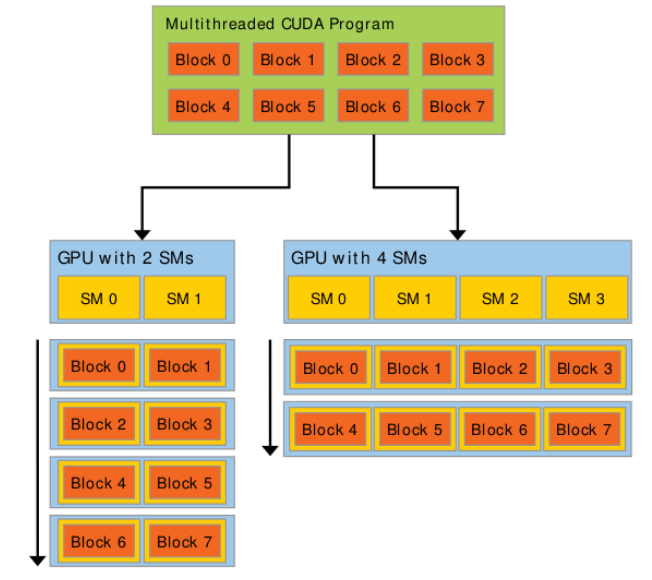
\includegraphics[width=0.8\textwidth]{images/cudaSMs.png}
		\caption{GPU scalability.}
		\label{fig:cudaSM}
	\end{figure}
	Indeed, \textit{each block of threads can be scheduled on any of the available Streaming Multiprocessors within a GPU, in any order, concurrently or sequentially}, such that a compiled CUDA program can execute on any number of SM, as illustrated by Figure \ref{fig:cudaSM}, and only the runtime system needs to know the physical multiprocessor count.
	This programming model scales on the number of multiprocessors and memory partitions \cite{cudaguide}. 
	
	We'll see in next \hyperref[sect:CUDAcpp]{section} further details on CUDA programming model, especially the extensions for C/C++ since, in this thesis, we used CUDA C++.
	
\subsection{Copy engines and Memory organization}
On all operating systems that run CUDA, host memory is virtualized. The operating system component that manages virtual memory is the \textit{Virtuam Memory Manager} (VMM), it provides services to hardware drivers, in order to facilitate direct access of host memory by hardware.\\
In modern computers, many peripheral, as GPUs, can read or write host memory using a facility known as \textbf{\textit{Direct Memory Access}} (\textbf{DMA}). It avoids a data copy and enables the hardware to operate concurrently with the CPU, furthermore hardware may achieve better bus performances over DMA.\\
To facilitate DMA, operating system VMMs provide a service named \textit{page-locking}. Page-locked memory is ineligible for eviction and its physical addresses cannot change. Once memory is page-locked, drivers can program their DMA hardware to reference the physical addresses of the memory.\\
Memory that isn't page-locked is known as \textit{pageable}, otherwise it's defined as \textbf{\textit{pinned}} memory\footnote{It's called \textit{pinned} since its physical addresses cannot be changed by the OS.}.\\
We'll see that \textbf{\textit{host pinned memory}}, with respect to the GPUs, is generally coupled with CUDA streams and it represents a page-locked portion of host memory, set up for DMA by the current CUDA context\footnote{To be precise page-locked memory and CUDA's pinned aren't really the same thing: pinned memory, registered by CUDA, is mapped for direct access by the GPU; ordinary page-locked memory is not.}.\\

We'll see in subsection \ref{subs:streams} CUDA Streams and we'll see that they are linked to DMA for another reason.
In particular, an important DMA mechanism is the so called \textbf{\textit{copy engine}}. \\
DMA allows the transfer of data between host and device, while eventually a kernel is executing on the GPU.\\
In older GPU architectures there was a single copy engine, while in newer there are usually 2.\\
The benefit of dual copy engines, coupled with the fact that PCIe\footnote{text} is a full duplex interconnection, allows to perform more operations simultaneously, for example:
\begin{itemize}
	\item do a memory copy from device to host;
	\item Run kernel that operates on available data in memory;
	\item do another memory copy from host to device.
\end{itemize}
\begin{figure}[H]
	%\vspace*{-2.4cm}
	\centering
	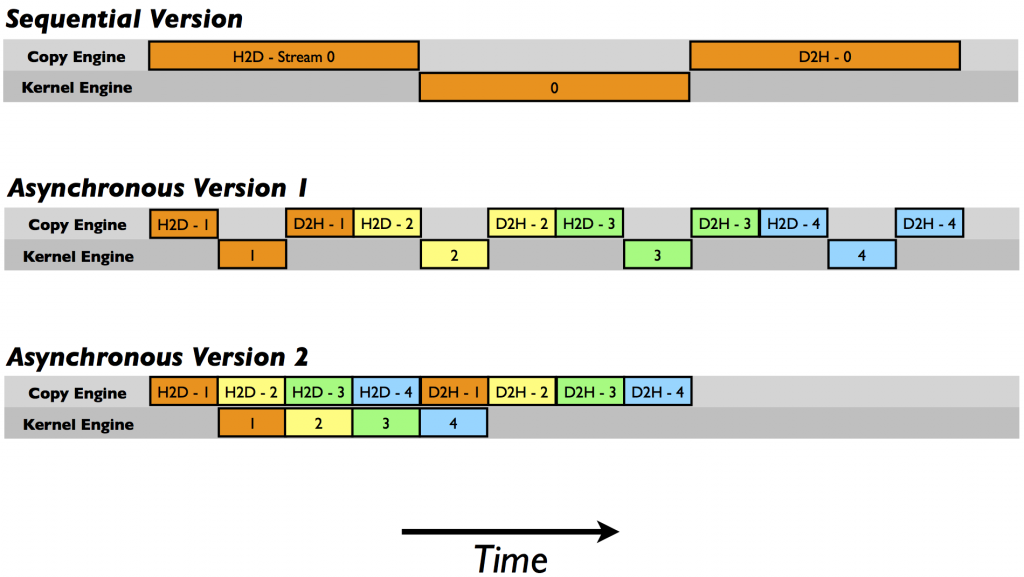
\includegraphics[width=0.8\textwidth]{images/streams-copy-engine.png}
	\caption{Comparison between no CUDA streams, one copy engine and streams, two copy engines and streams.}
	\label{fig:copyengines}
\end{figure}
In the ideal case, all data copies are completely overlapped by kernel execution, i.e. the transfers overheads are hidden by the kernel time\footnote{We'll see what overlapping really means and how it's implemented in subsection \ref{subs:streams}}.\\
With a single copy engine, instead, first and last steps above cannot run concurrently\footnote{Note that the simultaneous upload/download of large amounts of data across PCIe can use up a significant portion of available system memory bandwidth.}\cite{cudahandbook}.\\
In Figure \ref{fig:copyengines}, starting from the top, we have a comparison between the cases of: memory copies and kernel executions completely serial; memory copy and kernel execution overlapping (one copy engine); memory copies and kernel execution overlapping (two copy engines).\\
	
	
To maximize performance, CUDA uses different types of memory, depending on the expected usage.\\
As mentioned before, host memory refers to the memory attached to the CPU(s) in the system. Device memory is attached to the GPU and accessed by a dedicated memory controller and data should be copied explicitly\footnote{A new CUDA functionality, called \textit{Unified Memory} allows to abstract both device and host memories as if they are only one, this avoids the use of explicit copies between host and device memory. However this feature wasn't used in this work, as it wasn't suitable to allow tests and measures we needed to perform in experiments. } between host and device memory in order to be processed by the GPU.\\
Device memory can be allocated and accessed in different of ways:
\begin{itemize}
	\item \textbf{Global memory} may be allocated statically or dynamically and accessed via pointers in CUDA kernels, which translate to global load/store instructions;
	\item \textbf{Constant memory} is read-only memory accessed via different instructions that cause the read requests to be serviced by a cache hierarchy, optimized for broadcast to multiple threads;
	\item \textbf{Local memory} contains the stack, that is local variables that cannot be held in registers, parameters, and return addresses for subroutines;
	\item \textbf{Texture memory} (in the form of CUDA arrays) is accessed via texture and surface load/store instructions; like constant memory, read requests from texture memory are serviced by a separate cache that is optimized for read-only access.
\end{itemize}
Shared memory is an important type of memory in CUDA that is not supported by device memory. Instead, it is an abstraction for an on-chip memory that can be used for fast data interchange between threads within a block. Physically, shared memory comes in the form of built-in memory on the SM.\\
In this work we mainly exploited Global memory, it is the main abstraction by which CUDA kernels read or write device memory.\\
The device pointer base resides in the device address space, separate from the CPU address space used by the host code in the CUDA program. As a result, host code in the CUDA program can perform pointer arithmetic on device pointers, but they may not dereference them.\\
CUDA kernels can read or write global memory using standard C semantics such as pointer indirection (operator*, operator->) or array subscripting (operator[])\cite{cudahandbook}. 

	
\section{CUDA C/C++}
\label{sect:CUDAcpp}
Here we'll briefly introduce main concepts behind the CUDA programming model, by outlining how they are exposed in C.
Especially we'll show important notions about features involved in this project and how/why these were included.


\subsection{Kernels} 
\label{subs:ker}
CUDA C allows to define particular C functions, called \textbf{\textit{kernels}}.\\
when called, these are executed N times in parallel by N different CUDA threads, instead of executing only once, like it happens in regular C functions.

A kernel code is defined using the \texttt{\_\_global\_\_} declaration specifier. The number of CUDA threads that will execute the kernel for a given call is specified using this special execution configuration syntax: 
\texttt{<<<...>>>}.\\
Each thread executing the kernel is given a unique thread ID, accessible within the kernel through the built-in \texttt{threadIdx} variable\cite{cudaguide}.\\
\begin{wrapfigure}{l}{0.58\textwidth}
	\raggedleft
	
	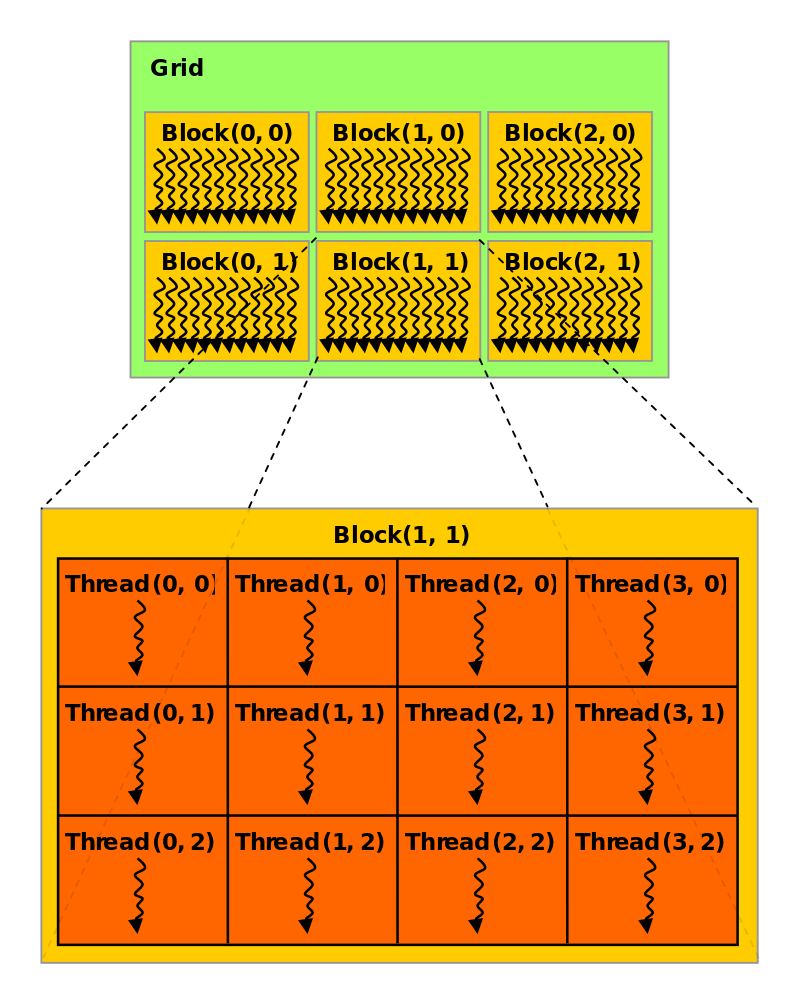
\includegraphics[width=0.58\textwidth]{images/gridblocks.png}
	\caption{Above: a Grid formed by Blocks.\\ Below: a Block formed by Threads.}
	\label{fig:gridblock}
\end{wrapfigure}

\subsection{Thread Hierarchy}  
\label{subs:thrhierarchy}
In practice \texttt{threadIdx} is a 3-component vector, so that threads can be identified using either one, or two, or three dimensional thread index.
In turn these threads will form	either one, or two, or three dimensional block of threads, called a
\textbf{\textit{thread block}}.
This provides a way to invoke computation across the elements in domains such as a vectors, matrices, or volumes.
%The index of a thread and its thread ID relate to each other in a straightforward way:
%\begin{itemize}
%	\item For a one-dimensional block, they are the same; 

%	\item for a two-dimensional block of size \((D_{x} ,	D_{y}) \space \rightarrow \space\)  a thread of index \((x, y)\) has \(threadID = (x + y \cdot D_{x} );\)

%	\item for a three-dimensional block of size \((D_{x} ,	D_{y} ,	D_{z}) \space \rightarrow \space\)  a thread of index \((x, y, z)\) has \(threadID = (x + y \cdot D_{x} + z \cdot D_{x} \cdot D_{y});\)
%\end{itemize}
There is a limit to the number of threads per block, since \textit{all threads of a block are expected to reside on the same processor core and must share the limited memory resources of that core}. On current GPUs, and on the two we worked on, a thread block may contain up to 1024 threads \footnote{see Table \ref{tab:gpuspecs} for limits in the machines we used).}.\\
However, a kernel can be executed by multiple equally-shaped thread blocks, so that\\
\(Total number of threads = \#threadsPerBlock \cdot \#blocks\)\\	 
Blocks in turn are organized into either one, or two, or three dimensional \textit{\textbf{grid of thread blocks}} as illustrated by Figure \ref{fig:gridblock}.	
So, the number of blocks in a grid is usually dictated by the size of the data being processed or the number of processors in the system.
The number of \textit{threads per block} and the number of \textit{blocks per grid} specified in the 	\texttt{<<<...>>>} syntax can be of type \texttt{int} or \texttt{dim3}.\\
The dimension of the thread block, block index and thread index are accessible within the kernel through the respective built-in variables: \texttt{blockDim}, \texttt{blockIdx}, \texttt{threadIdx}. \cite{cudaguide}.

\subsection{CUDA Streams}
\label{subs:streams} 
CUDA is best known for enabling fine-grained concurrency, with hardware facilities that enable threads to closely collaborate within blocks, using a combination of shared memory and thread synchronization.\\
But it also has hardware and software facilities that enable more \textit{coarse-grained concurrency}: 
\begin{itemize}
	\item \textit{CPU/GPU concurrency}. Since they are separate devices, the CPU and GPU can operate independently of each other;
	\item \textit{Memcpy/kernel processing concurrency}. For GPUs that have one or more copy engines, \(host \leftrightarrow device\) memcpy can be performed while the SMs are processing kernels;
	\item \textit{Kernel concurrency}. SM, in 2.x compute capability and later hardware, can run up to 4 kernels in parallel;
	\item \textit{Multi-GPU concurrency}. For problems with enough computational density, multiple GPUs can operate in parallel.
\end{itemize}
  CUDA streams enable these types of concurrency, but we're interested mainly in the first three types listed above.\\
  Within a given stream, operations are performed in sequential order, but operations in different streams may be performed in parallel.\\
  CUDA events complement CUDA streams by providing the synchronization mechanisms needed to coordinate the parallel execution enabled by streams. CUDA events may be used for CPU/GPU synchronization, for synchronization between the engines on the GPU, and for synchronization between GPUs.\\
  They also provide a GPU-based timing mechanism that cannot be perturbed by system events such as page faults or interrupts from disk or network controllers \cite{cudahandbook}. \\
  

	\textbf{Overlap of Data Transfer and Kernel Execution}\\
	Some devices can perform an asynchronous memory copy to or from the GPU	concurrently with kernel execution. 
	It's possible to query this capability by checking the \texttt{asyncEngineCount} device property \footnote{ See \textit{Device Enumeration} in Table \ref{tab:gpuspecs}, for both of our machines, from the \textit{deviceQuery}, we get 2 copy engines.}, which is greater than zero for devices that support it.


	When host memory is involved in the asynchronous copy, it must be
	\textit{\textbf{page-locked}} to possibly achieve a kernel-copy overlap\cite{cudastrandconcurr}.\\
	
	
	%In particular some devices, of compute capability 2.x and higher, can overlap copies to and from the device. Applications may query this capability by checking the \texttt{asyncEngineCount} device property (see Device Enumeration), which is equal to 2 for devices that support	it \footnote{This is the case for both of our machines. \\ See the last line of \texttt{deviceQuery} in Table \ref{tab:gpuspecs}}. 
	%\Large \textbf{Streams}\normalsize\\
	
	Applications manage the concurrent operations described above through \textbf{CUDA streams}. A stream is a sequence of commands (possibly issued by different host threads) that execute in order. On the other hand, a stream may execute their commands out of order or concurrently with respect to another; this behavior is not guaranteed and	should not be relied upon for correctness (e.g. inter-kernel communication is undefined)\cite{cudaguide,custreamsblog}.\\
	A brief code example:
	\begin{lstlisting}[caption={CUDA Strams creation}]
	cudaStream_t stream[2];
	for (int i = 0; i < 2; ++i)
	cudaStreamCreate(&stream[i]);
	float* hostPtr;
	cudaMallocHost(&hostPtr, 2 * size);
	\end{lstlisting}	
	
	Each of these streams is defined, by the following code sample, as a sequence of one memory copy \(host \rightarrow device\), one kernel launch, and one memory copy \(host \leftarrow device\):
	\begin{lstlisting}[caption={CUDA Strams and Async example}]
	for (int i = 0; i < 2; ++i) {
	cudaMemcpyAsync(inputDevPtr + i * size, hostPtr + i * size, size, cudaMemcpyHostToDevice, stream[i]);
	MyKernel <<<100, 512, 0, stream[i]>>> (outputDevPtr + i * size, inputDevPtr + i * size, size);
	cudaMemcpyAsync(hostPtr + i * size, outputDevPtr + i * size, size, cudaMemcpyDeviceToHost, stream[i]);
	}
	\end{lstlisting}
	
	Each stream copies its portion of input array \texttt{hostPtr} to array \texttt{inputDevPtr} in device memory, processes \texttt{inputDevPtr} on the device by calling \texttt{MyKernel()}, and copies
	the result \texttt{outputDevPtr} back to the same portion of \texttt{hostPtr}. Note that \texttt{hostPtr} must point to page-locked host memory for any overlap to
	occur.\\
	Streams are released by calling \texttt{cudaStreamDestroy()}.
	\begin{lstlisting}[caption={CUDA Strams destroy}]
	for (int i = 0; i < 2; ++i)
	cudaStreamDestroy(stream[i]);
	\end{lstlisting}


\subsection{nvcc compiler}
	To compile the CUDA C++ code it is necessary to use a special compiler, included in CUDA Toolkit, that is \texttt{nvcc}.\\
	The CUDA compiler driver hides the details of CUDA compilation from developers. It accepts a range of conventional compiler options, for example for the project we could define macros or include library paths \footnote{NVCC documentation: https://docs.nvidia.com/cuda/cuda-compiler-driver-nvcc/index.html\#introduction}.\\ 
	All non-CUDA compilation steps are forwarded to a C++ host compiler that is supported by \texttt{nvcc}. 
	Source files compiled with \texttt{nvcc} can include a mix of host code and device code. \texttt{nvcc}'s basic
	workflow consists in separating device from host code and then:
	\begin{itemize}
		\item compiling the device code into an assembly form (PTX code) and/or binary form (cubin object), \item and modifying the host code by replacing the \texttt{<<<...>>>} syntax introduced in	Kernels \footnote{See  \hyperref[subs:ker]{subsection 2.3.1}} by the necessary CUDA C runtime function calls, to load and launch each compiled kernel from the PTX code and/or cubin object.
	\end{itemize}
	The modified host code is output either as C code that is left to be compiled using another tool, or as object code directly by letting \texttt{nvcc} invoke the host compiler during	the last compilation stage.
	Applications can then either link to the compiled host code (most common case), or ignore the modified host code (if any) and use the CUDA driver API to load and execute the PTX code or cubin object.\\
	This compiler can be used almost the same way as a classic \texttt{gcc}, for example:
	
	\texttt{nvcc -std=c++14 -g -G -o exec source.cu}\\
	This is an example that compiles the file \texttt{source.cu} in the executable file \texttt{exec}, keeping debug information with \texttt{-g -G} flags.
	Here we present compiler versions installed in our two machines:	
	\begin{itemize}
		\item \textbf{Tesla P100}\\
		nvcc: NVIDIA (R) Cuda compiler driver, release 10.1, V10.1.168			
		
		\item \textbf{Tesla M40}\\
		nvcc: NVIDIA (R) Cuda compiler driver, release 10.1, V10.1.105
	\end{itemize}

	\subsection{\texttt{cuda-gdb} debugger}
	\texttt{CUDA-GDB} is the NVIDIA tool for debugging CUDA applications (available on Linux). It is an extension to the x86-64 port of GDB, the GNU Project debugger.\\
	\texttt{CUDA-GDB} main features are:
	\begin{itemize}
		\item it provides an environment that allows simultaneous debugging of both GPU and CPU code within the same application;
		
		\item as programming in CUDA C is an extension to C programming, debugging with CUDA-GDB is an extension to debugging with GDB, so the existing GDB debugging features are present for debugging the host code (additional features have been provided to support  CUDA device code);	
		
		\item it allows to set breakpoints, to single-step CUDA applications, and also to inspect and modify the memory and variables of any given thread running on the hardware;
		
		\item it supports debugging all CUDA applications, whether they use the CUDA driver API, the CUDA runtime API, or both.
		
		\item it supports debugging kernels that have been compiled for specific CUDA architectures, but also supports debugging kernels compiled at runtime, referred to as just-in-time (JIT) compilation.
	\end{itemize}	
	\texttt{CUDA-GDB} was used to debug all compiled source files, both \texttt{.cu} and \texttt{.cpp} .
	Mainly it was really helpful in this project to step device code, inspect runtime errors thrown by CUDA API calls and check exactly what code was doing inside our kernels.





\section{Profilers}	
	NVIDIA profiling tools were useful to optimize performances of our CUDA applications.\\
	We used two different versions, that will be showed in the following sections.
		
	\subsection{nvprof}
	The\texttt{nvprof} provides a tool to collect and view profiling data from the command-line.
	\texttt{nvprof} was added to CUDA Toolkit with CUDA 5. It is a command-line profiler, so it's a GUI-less version of the graphical profiling features available in the NVIDIA Visual Profiler.\\
	The \texttt{nvprof} profiler enables the collection of a timeline of CUDA-related activities on both CPU and GPU, including kernel execution, memory transfers, memory set and CUDA API calls and events or metrics for CUDA kernels.\\
	After all data is collected, profiling results are displayed in the console \footnote{The textual output of the profiler is redirected to \texttt{stderr} by default.} or can be saved in a log file for later viewing \footnote{Or for later import into either \texttt{nvprof} or the \texttt{NVIDIA Visual Profiler)}.} \cite{profilersguide, nvprofarticle}.\\
	\texttt{nvprof} operates in different modes: \textit{Summary Mode}, \textit{GPU-Trace and API-Trace Modes}, \textit{Event/metric Summary Mode} and  \textit{Event/metric Trace Mode}.\\	
	For our purposes we used only \textit{Summary Mode}, this is the default operating mode, where we have a single result line for each kernel function and each type of CUDA memory copy performed by the application (for each operation type are shown number of calls and total, max, min and average time) \cite{profilersguide}.
	
	We used it, in some situations, as a quick check, for example we exploited it to see if the application wasn't running kernels on the GPU at all, or it was performing an unexpected number of memory copies, etc.
	To this aim it's enough to run the application with\\
	\texttt{nvprof ./myApp arg0 arg1 ...}\\
	Given that we wanted to consult profiling results whenever it was necessary, we used \texttt{--log-file} option to redirect the output to files for deferred examination. \\
	\texttt{nvprof} revealed peculiarly suitable for remote profiling. That's because of the fact command line is faster to check and save an application profiling.
	  
	\subsection{NVIDIA Visual Profiler}
	The NVIDIA Visual Profiler, introduced in 2008, is a performance profiling tool providing visual feedback for optimizing CUDA C/C++ applications.
	
	The Visual Profiler displays a timeline of an application's activity on both the CPU and GPU to make performance improvement, it analyzes the application to detect potential bottlenecks, using graphical views, that allow to check memory transfers, kernel launches, and other API functions on the same timeline \cite{profilersguide}.\\
	 
	\texttt{Visual Profiler} was also used in developing phase, to check if code was properly written to hide as much as possible data transfers \footnote{We'll see in detail the Overlapping topic and how it was managed in \hyperref[chap:logic]{Chapter 3}.}, even though sometimes it may happen that profilers introduce some sampling synchronization, giving some little imprecision in visual results.

	
\section{Visual Studio Code}
	Visual Studio Code is an open-source code editor by Microsoft that also runs on Linux Operating Systems. It includes support for debugging, embedded Git control and GitHub, syntax highlighting, intelligent code completion, snippets, and code refactoring \footnote{Other infos: https://en.wikipedia.org/wiki/Visual\_Studio\_Code \\
		Documentation: https://docs.microsoft.com/it-it/dotnet/core/tutorials/with-visual-studio-code \\ 
		Website: https://code.visualstudio.com/}.\\
	Since it's customizable we could add C++ and CUDA editor extensions, furthermore an SFTP extension allowed us to quickly upload/download files from remote machines. 	
	
	
\section{Tests, Result gathering, Plots}
	Some other additional tools have been used in this project.
	In particular we needed:
	\begin{itemize}
		\item to serially run executions of our applications, possibly varying input dataset on interest values;
		\item to group all results on text files;
		\item to implement a script to compute averages, speedups and other interest metrics, from results on text files;
		\item a generator of graphs on important values from the obtained calculations.
	\end{itemize}
	
	\subsection{Bash scripts}
	\label{subs:bash}
	Bash (Bourne-Again SHell) is the shell, or command language interpreter, for the GNU operating system; the latter provides other shells, but Bash is the default  shell\footnote{https://www.gnu.org/software/bash/manual/}. 
	
	\textbf{\texttt{Bash scripts}} were needed to implement tests, that run more executions of a certain CUDA application, also varying input dataset.
	We programmed bash scripts (\texttt{.sh}) tests to contain several command as compile a certain CUDA application, run many times the related executable, profile it with \texttt{nvprof} and so on.\\
	Below we give a brief example on how we used bash scripts to implement tests:
	\begin{lstlisting}[caption={Tests on bash scripts example},language=bash]
	#!/bin/bash
	
	...			
	let GPU=3
	let B=1024
	let nTests=4

	Miters=(10000 400000 800000)
	Ns=(57344 114688 229376 458752 917504 1835008)
		
	#parameters: deviceID, BLOCK, N_elements, M_iterations, cuStr[bool], strNum
	make cleandplow
	echo -e "${BLUE}compiling stream...${NC}"
	
	make streamlow
	
	echo ***STREAM_LOW_NOSTREAM_test***

	for N in "${Ns[@]}"
	do			
		for m in "${Miters[@]}"
		do	
			echo sizeN = $N elements, kerM = $m , CUstreams = 0 
			echo -n execIndex = 
			
			for((j=0; j<nTests; j+=1));
			do
				echo -n "$j , "
				./bin/streamlow.out $GPU $B $N $m 0 0 >> ./results/dev_cos_dp_stl.txt
			done
			echo -ne "$nTests \n"			
			nvprof --log-file ./profiling/dev_str_low$N-$m-$B-0.txt ./bin/streamlow.out $GPU $B $N $m 0 0 >> ./results/dev_cos_dp_stl.txt
		done
	done
	\end{lstlisting}
	Here, for example, the code is setting up all input data set, it compiles the code with the \texttt{streamlow} rule into an executable, then it loops over all data sets to run the executable in each configuration.\\
	Here we can see that each setting is repeated more times (to allow outliers elimination) and one of those executions is performed via the \texttt{nvprof} profiler, in any case all outputs are redirected to consultable \texttt{.txt} files.
	
	
	\subsection{Python scripts}
	As Python \footnote{The Python version used to compile, on local host, our scripts is: Python 2.7.6.\\ See documentation: https://docs.python.org/2/} has dynamic typing, together with its interpreted nature, it's an ideal language for scripting and rapid application development.
	
	In the case of this work was most useful to quickly implement a result filter: given text files with time measures, we computed averages and some speedups. \\
	Furthermore we implemented a script to generate some plots on averages and speedups, exploiting the library \texttt{matplotlib}\footnote{https://matplotlib.org/}.\\
	Below we show a part of the code to compute speedups and generate some plots:
	\begin{lstlisting}[caption={Portion of speedup and plots Python script}, language=python]
	def main():		
		res_path = "./output/"+sys.argv[1]+"/"
		for file in os.listdir(res_path):
			if file.endswith("avgs.csv"):
				f=os.path.join(res_path, file)
				
				resType=file[0:3]
				if resType=="cos":
					dataPar,zeroStream,threeStream,coresStream = getDividedData(dpCosTest,strCosTest,f)	
				elif resType=="mat":
					dataPar,zeroStream,threeStream,coresStream = getDividedData(dpMatTest,strMatTest,f)	
				...
				
				zeroThree,zeroCore,coreDp = getSpeedup(zeroStream,threeStream,coresStream,dataPar)				
				
				csvPath=res_path+resType+"_sp.csv"
				##write speedup to CSV##
				with open(csvPath,  "wb") as fcsv:
					writer = csv.writer(fcsv) 					
					printSpToCSV("Tseq/T3",zeroThree,resType,writer) #num, size, time
					printSpToCSV("Tseq/Tsm",zeroCore,resType,writer)
					printSpToCSV("Tsm/Tdata",coreDp,resType,writer)
			
				#########
				# Plots #
				#########
				# Completion Time
				launchPlots(resType,zeroStream,"Zero Streams")
				launchPlots(resType,threeStream,"Three Streams")
				launchPlots(resType,coresStream,"#SM Streams")
				# Speedup	
				streamNums=[]
				if sys.argv[1]=="M40":
					streamNums=[1,3,24]
				elif sys.argv[1]=="P100":
					streamNums=[1,3,56]				
				
				if resType=="cos":
					plotSpeedup(streamNums, zeroStream, zeroThree, zeroCore, resType, cosN, cosM)	
				elif resType=="mat":
					plotSpeedup(streamNums, zeroStream, zeroThree, zeroCore, resType, matNum, matSize)		
				...
				
	#########################
	# Speedup plot function #
	#########################
	def plotSpeedup(streamNums,zeroStream, zeroThree , zeroCore, resType,param1,param2):				
		title="Speed Up"		
		title=title.upper()	
			
		plt.figure(figId)
		plt.plot([0]+streamNums, [0]+streamNums, marker='.',label='Ideal speed up',linestyle='--')
		
		tmp=[]
		j=0
		lineW=0.5
		alphaVal=1.0
		if resType=="cos":
			indexes=[0, param2-1, len(zeroCore)-param2, len(zeroCore)-1]
			for i in indexes:
				tmp=[1.0, zeroThree[i][2],zeroCore[i][2]]
				lblLine=str(zeroThree[i][0]) +" - "+str(zeroCore[i][1])
				plt.plot(streamNums, tmp, '-', label = lblLine, marker=markers[j], linestyle='-', linewidth=lineW, alpha=alphaVal)
				
				lineW+=0.5
				alphaVal-=0.2
				j+=1
		...
		
		plt.xticks(streamNums)
		plt.yticks(streamNums)
		plt.legend(loc="upper left")
		plt.grid(axis='both')
		plt.ylabel("Speedup")
		plt.xlabel("#CUDA Streams")
		plt.show()
		plotId+=1
		figId+=1
	\end{lstlisting}
	
	The code above starts in function \texttt{main()}, it initially reads from a \texttt{.csv} the average time measures for all types of execution by one of the three applications we tested.\\
	Then in the main we split times of all execution types (e.g. zero, three or number of SM amount of CUDA streams used). At this point code has what it needs to get all speedups\footnote{We'll see in Chapter \ref{chap:experim} all types of speedup we compute, how and why.} in \texttt{getSpeedup}, this function computes speedup (from input parameters) then it saves results in a \texttt{.csv} file and output them to the main function too.\\
	Finally the main calls the functions that provide completion time and speedup plots, respectively called \texttt{launchPlots} and \texttt{plotSpeedup}. The latter plots all different speedups, given by the different input data sets of executions, compared with the line of ideal speedup.
	

